\chapter{Introduction to Elder Topology}

\begin{chapterabstract}
This chapter presents the topological framework that connects abstract Elder spaces to practical applications through realization mappings. We develop phase-coherent manifolds that bridge theoretical structures with observable phenomena in specific domains. The topological properties of Elder spaces—including their phase-preserving homomorphisms, spectral invariants, and stratification—explain fundamental mechanisms like resonance and cross-domain transfer. This mathematical foundation establishes Elder Theory as a rigorous formalism with precise guarantees for knowledge representation and transfer capabilities.
\end{chapterabstract}

\section{Topological Structure}

Elder spaces possess a natural topology that arises from their algebraic structure and phase properties.

\begin{definition}[Elder Topology]
The topology on an Elder space is based on the product topology of the parameter space and phase space. The basic open sets include both parameter proximity and phase alignment considerations.
\end{definition}

\begin{theorem}[Topological Properties]
An Elder space with its natural topology forms a well-behaved mathematical space that supports continuity of the knowledge transfer operations essential to the theory.
\end{theorem}

\begin{definition}[Resonance Manifold]
A subset $\mathcal{M}$ of an Elder space is a resonance manifold if it represents a collection of elements that maintain consistent phase relationships when parameter values change. These manifolds provide the mathematical structure for knowledge transfer across domains.
\end{definition}

\begin{theorem}[Stratification]
Every Elder space admits a canonical stratification into phase-coherent manifolds:
\begin{equation}
\elder{d} = \bigcup_{k=0}^{d} \mathcal{S}_k
\end{equation}
where each $\mathcal{S}_k$ is a disjoint union of $k$-dimensional phase-coherent manifolds.
\end{theorem}

\begin{figure}[ht]
\centering
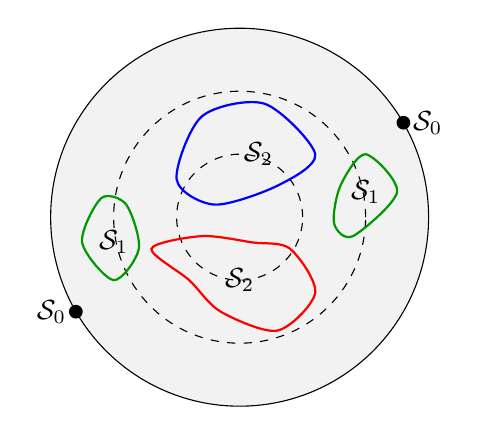
\begin{tikzpicture}[scale=0.8]
\draw[fill=black!5] (0,0) circle (3);
\draw[thin, dashed] (0,0) circle (2);
\draw[thin, dashed] (0,0) circle (1);

\draw[blue, thick] plot [smooth cycle] coordinates {(0.6,0.5) (1.2,1.0) (0.4,1.8) (-0.6,1.6) (-1.0,0.6) (-0.4,0.2)};
\node at (0.3,1.0) {$\mathcal{S}_2$};

\draw[red, thick] plot [smooth cycle] coordinates {(-1.4,-0.5) (-0.8,-1.0) (-0.3,-1.5) (0.6,-1.8) (1.2,-1.2) (0.8,-0.5) (0.2,-0.4) (-0.6,-0.3)};
\node at (0,-1.0) {$\mathcal{S}_2$};

\draw[green!60!black, thick] plot [smooth cycle] coordinates {(-2.2,0.3) (-2.5,-0.4) (-2.0,-1.0) (-1.6,-0.5) (-1.8,0.2)};
\node at (-2.0,-0.4) {$\mathcal{S}_1$};

\draw[green!60!black, thick] plot [smooth cycle] coordinates {(1.8,-0.3) (2.5,0.4) (2.0,1.0) (1.6,0.5) (1.5,-0.1)};
\node at (2.0,0.4) {$\mathcal{S}_1$};

\filldraw (2.6, 1.5) circle (0.1) node[right] {$\mathcal{S}_0$};
\filldraw (-2.6, -1.5) circle (0.1) node[left] {$\mathcal{S}_0$};
\end{tikzpicture}
\caption{Stratification of Elder space into phase-coherent manifolds}
\label{fig:elder-stratification}
\end{figure}

This stratification is fundamental to understanding the dynamics of Elder learning processes, as each stratum corresponds to states with similar structural properties.

\section{Realization Mappings}

Realization mappings connect abstract Elder spaces to measurable phenomena in specific domains.

\begin{definition}[Realization Mapping]
A realization mapping $\realization{X}: \elder{d} \rightarrow \mathcal{F}(X)$ from an Elder space to a function space over domain $X$ is a continuous mapping that preserves phase and spectral structure.
\end{definition}

\begin{theorem}[Universal Realization]
For any Elder space $\elder{d}$, there exists a canonical realization mapping $\realization{U}: \elder{d} \rightarrow L^2(U_d)$ that is:
\begin{enumerate}
    \item Injective: $\realization{U}(x) = \realization{U}(y) \implies x = y$
    \item Additive: $\realization{U}(x \oplus y) = \realization{U}(x) + \realization{U}(y)$
    \item Multiplicative: $\realization{U}(x \star y) = \realization{U}(x) \cdot \realization{U}(y)$
    \item Phase-preserving: $\Phi(x) = \Phi_{\mathcal{F}}(\realization{U}(x))$
\end{enumerate}
\end{theorem}

This theorem establishes that every abstract Elder space can be faithfully represented in a concrete functional space, preserving all relevant algebraic and phase properties.

\section{Spectral Properties}

The spectral properties of Elder spaces provide deep insights into their structure and behavior.

\begin{definition}[Spectral Bundle]
The spectral bundle of an Elder space is $\mathcal{E}_d = \elder{d} \times_{\Phi} \mathbb{S}^1$, whose fiber over each point of $\mathbb{S}^1$ consists of all elements with the corresponding phase.
\end{definition}

\begin{lemma}[Spectral Realization]
For any $x \in \elder{d}$ with spectral decomposition $x = \sum_{i=1}^{d} \lambda_i e^{i\theta_i} \odot \elderstructure{i}$, the realized function $\realization{X}(x)$ has:
\begin{enumerate}
    \item Norm: $\|\realization{X}(x)\|_{L^2} = \sqrt{\sum_{i=1}^{d} \lambda_i^2}$
    \item Phase: Weighted combination of the phases $\theta_i$ at each point
    \item Resonance: Amplification where phases $\theta_i$ align coherently
\end{enumerate}
\end{lemma}

\begin{theorem}[Topological Invariants]
The spectral bundle $\mathcal{E}_d$ admits topological invariants that completely characterize its structure:
\begin{enumerate}
    \item Chern classes $c_k(\mathcal{E}_d) \in H^{2k}(\mathbb{S}^1, \mathbb{Z})$
    \item A canonical flat connection $\nabla_E$ with holonomy group $U(1)^d$
    \item The characteristic Elder class $\chi_E(\mathcal{E}_d)$
\end{enumerate}
\end{theorem}

These invariants provide a complete topological classification of Elder spaces, enabling structural analysis of their properties.

\section{Hierarchical Structure and Transfer}

The hierarchical structure of Elder spaces leads naturally to a theory of cross-domain knowledge transfer.

\begin{theorem}[Hierarchical Realization]
The Elder-Mentor-Erudite hierarchy induces corresponding domain realizations:
\begin{align}
\realization{\mathcal{D},E}: \eldersubspace &\rightarrow \mathcal{F}_E(\mathcal{D}) \\
\realization{\mathcal{D},M}: \mentorsubspace &\rightarrow \mathcal{F}_M(\mathcal{D}) \\
\realization{\mathcal{D},Er}: \eruditesubspace &\rightarrow \mathcal{F}_{Er}(\mathcal{D})
\end{align}
representing increasingly concrete functional representations of domain knowledge.
\end{theorem}

\begin{corollary}[Cross-Domain Transfer]
For domains $\mathcal{D}_1$ and $\mathcal{D}_2$, the transfer operator:
\begin{equation}
\mathcal{T}_{\mathcal{D}_1 \rightarrow \mathcal{D}_2} = \realization{\mathcal{D}_2} \circ \realization{\mathcal{D}_1}^{-1}
\end{equation}
defines a rigorous mechanism for knowledge transfer between domains.
\end{corollary}

This formalism establishes the mathematical foundation for Elder Theory's cross-domain knowledge transfer capabilities, providing a precise mechanism for how information learned in one domain can be applied to another.

\section{Resonance Geometry}

The topological framework reveals resonance as a fundamental geometric property of Elder spaces.

\begin{definition}[Resonance Manifold]
For elements $x, y \in \elder{d}$, the resonance manifold is:
\begin{equation}
\mathcal{R}(x, y) = \{z \in \elder{d} \mid \Phi(x \star z) = \Phi(y \star z)\}
\end{equation}
\end{definition}

\begin{theorem}[Resonance Structure]
Resonance manifolds $\{\mathcal{R}(x, y)\}$ foliate the Elder space, with learning dynamics naturally flowing along these manifolds toward states of increasing phase coherence.
\end{theorem}

The geometry of resonance manifolds explains how the Elder-Mentor-Erudite system naturally discovers coherent structures across domains, providing a mathematical foundation for its emergent learning behaviors.

\section{Connections to Dynamical Systems}

Elder topology establishes profound connections to dynamical systems theory.

\begin{theorem}[Symmetry Correspondence]
The Elder space spectral bundle exhibits symmetry properties similar to dynamical systems, where:
\begin{enumerate}
    \item Structural elements correspond to fundamental system modes
    \item The phase operator corresponds to cycle dynamics
    \item Resonance manifolds correspond to submanifolds of constructive interference
\end{enumerate}
\end{theorem}

\begin{theorem}[Phase Dynamics]
The Elder space phase structure induces a natural $U(1)^d$ symmetry group, where:
\begin{enumerate}
    \item Phase components are degrees of freedom
    \item Phase-coherent flows are covariant dynamics
    \item Resonance manifolds are invariant observables
\end{enumerate}
\end{theorem}

These connections reveal Elder Theory as a mathematical framework with deep ties to dynamical systems theory, suggesting that hierarchical learning systems share essential properties with complex systems that exhibit emergent behavior.

The topological framework established in this chapter provides the mathematical foundation for understanding how abstract Elder spaces connect to concrete domains, explaining the system's core capabilities of efficient knowledge representation, hierarchical organization, and cross-domain transfer.